\documentclass[10pt,a4paper]{report}
\usepackage[utf8x]{inputenc}
\usepackage{ucs}
\usepackage{amsmath}
\usepackage{amsfonts}
\usepackage{amssymb}
\usepackage{graphicx}
\author{Andraž Vrhovec}
\title{MRNA - seminar 1}
\begin{document}
\maketitle

\section{Hiter opis}

Imamo semafor z N luckami, kjer je ob zacetku igre prizgana srednja luc. V igri sodelujeta dva igralca, ki izmenicno pritiskatat tipki R1 ($alpha=1$) in R2 ($alpha=2$). Ob pritisku na tipko R1 se lucka premakne levo z verjetnostjo $p$ in desno z verjetnostjo $p-1$. Ob pritisku na R2 se lucka premakne levo z verjetnostjo $p-1$ in desno z verjetnostjo $p$. Cilj prvega igralca je lucko spraviti na skrajni levi rob semaforja, cilj drugega igralca pa na desni rob, pri cemer nihce ne ve verjetnosti $p$.

\section{Primerjava avtomatov z PCA}

Najprej sem vse avtomate primerjal z PCA. V vsaki primerjavi sem izvedel 100 ponovitev z maksimalnim stevilom korakov 1000. Pricakovano se je izkazalo da vecja kot je verjetnost p, boljse je ucenje avtomata in da se pri vrednostih $p$ blizu 0.5 avtomati obnasajo podobno kot PCA. Opaziti je tudi da pri majhnem N, lahko dodatni pomnilnik pri $L_{2n,2}$ skoduje procesu ucenja. Vrednosti -1 v tabeli pomenijo da se simulacija ni izvedla v doglednem casu, zato sem jo prekinil.


\begin{figure}[h!]
\begin{center}
\begin{tabular}{|c|c|c|c|c|}
\hline • & $L_{2,2}$ & $L_{6,2}$ & $L_{r-p}$ & $L_{r-i}$ \\ 
\hline PCA & 1,27 & 1,13 & 1,56 & 1,22 \\ 
\hline 
\end{tabular} 
\end{center}
\caption{Razmerje zmag ($\frac{|avtomat_i|}{|PCA|}$ pri N=7 in p=0,6}
\end{figure}

\begin{figure}[h!]
\begin{center}
\begin{tabular}{|c|c|c|c|c|}
\hline • & $L_{2,2}$ & $L_{6,2}$ & $L_{r-p}$ & $L_{r-i}$ \\ 
\hline PCA & 2,33 & 1,32 & 1,94 & 1,32 \\ 
\hline 
\end{tabular} 
\end{center}
\caption{Razmerje zmag ($\frac{|avtomat_i|}{|PCA|}$ pri N=7 in p=0,8}
\end{figure}

\begin{figure}[h!]
\begin{center}
\begin{tabular}{|c|c|c|c|c|}
\hline • & $L_{2,2}$ & $L_{6,2}$ & $L_{r-p}$ & $L_{r-i}$ \\ 
\hline PCA & 1,38 & 1,56 & 1,33 & 1,27 \\ 
\hline 
\end{tabular} 
\end{center}
\caption{Razmerje zmag ($\frac{|avtomat_i|}{|PCA|}$ pri N=19 in p=0,6}
\end{figure}

\begin{figure}[h!]
\begin{center}
\begin{tabular}{|c|c|c|c|c|}
\hline • & $L_{2,2}$ & $L_{6,2}$ & $L_{r-p}$ & $L_{r-i}$ \\ 
\hline PCA & 11.5 & 32,33 & 6,14 & 6,14 \\ 
\hline 
\end{tabular} 
\end{center}
\caption{Razmerje zmag ($\frac{|avtomat_i|}{|PCA|}$ pri N=19 in p=0,8}
\end{figure}

\begin{figure}[h!]
\begin{center}
\begin{tabular}{|c|c|c|c|c|}
\hline • & $L_{2,2}$ & $L_{6,2}$ & $L_{r-p}$ & $L_{r-i}$ \\ 
\hline PCA & $3,62$ & $91$ & $-1$ & $-1$ \\ 
\hline 
\end{tabular} 
\end{center}
\caption{Razmerje zmag ($\frac{|avtomat_i|}{|PCA|}$ pri N=101 in p=0,6}
\end{figure}

\begin{figure}[h!]
\begin{center}
\begin{tabular}{|c|c|c|c|c|}
\hline • & $L_{2,2}$ & $L_{6,2}$ & $L_{r-p}$ & $L_{r-i}$ \\ 
\hline PCA & $\infty$ & $\infty$ & $\infty$ & $\infty$ \\ 
\hline 
\end{tabular} 
\end{center}
\caption{Razmerje zmag ($\frac{|avtomat_i|}{|PCA|}$ pri N=101 in p=0,8}
\end{figure}

\section{Primerjva avtomatov med seboj}

Primerjava avtomatov med seboj je bila izvedena podobno kot primerjava z PCA, le da so se tokrat kot drugi igralec izmenjevali razlicni avtomati. Primerjati enak avtomat z enakim se mi ni zdelo smiselno, saj oba zavzameta podobne strategije in je izzid odvisen samo od srece.

\begin{figure}[h!]
\begin{center}
\begin{tabular}{|c|c|c|c|c|}
\hline • & $L_{2,2}$ & $L_{6,2}$ & $L_{r-p}$ & $L_{r-i}$ \\ 
\hline $L_{2,2}$ & • & 0,75 & 0,59 & 0,72 \\ 
\hline $L_{6,2}$ & • & • & 1,13 & 0.78 \\ 
\hline $L_{r-p}$ & • & • & • & 1,17 \\ 
\hline $L_{r-i}$ & • & • & • & • \\ 
\hline 
\end{tabular} 
\end{center}
\caption{Razmerje zmag ($\frac{|avtomat_zgoraj|}{|avtomat_levo|}$ pri N=7 in p=0,8}
\end{figure}

\begin{figure}[h!]
\begin{center}
\begin{tabular}{|c|c|c|c|c|}
\hline • & $L_{2,2}$ & $L_{6,2}$ & $L_{r-p}$ & $L_{r-i}$ \\ 
\hline $L_{2,2}$ & • & 3,55 & 1,63 & 0,82 \\ 
\hline $L_{6,2}$ & • & • & 0,47 & 0.78 \\ 
\hline $L_{r-p}$ & • & • & • & 0,19 \\ 
\hline $L_{r-i}$ & • & • & • & • \\ 
\hline 
\end{tabular} 
\end{center}
\caption{Razmerje zmag ($\frac{|avtomat_zgoraj|}{|avtomat_levo|}$ pri N=19 in p=0,8}
\end{figure}

\section{Primerjava parametrov korekcijskih shem}

V prvem primeru sem primerjal dva $L_{r-p}$ avtomata z razlicnimi parametri. Pri avtomatu z vecjimi parametri se vidi vecje odklone v verjetnosti izbire skozi cas, vedar se proti koncu ujameta kar se vidi tudi na razmerju zmag, ki je na koncu blizu 1.

V drugem primeru sem primerjal $L_{r-p}$ z $L_{r-i}$ z enakim a. Visi se veliko lepse ucenje $L_{r-i}$ avtomata, kar se pozna tudi na koncnem razmerju zmag $95:5$. Iz teh rezultatov zaklucujem da je $L_{r-i}$ avtomat boljsi za okolja kjer je verjetnost kaznovanja fiksna, vendar neznana. Dopuscam moznost da se $L_{r-p}$ boljse obnasa v dinamicnih okoljih, kjer se verjetnost kaznovanja spreminja, saj je njegov proces ucenja bolj fleksibilen v obe smeri.

\begin{figure}[h!]
\begin{center}
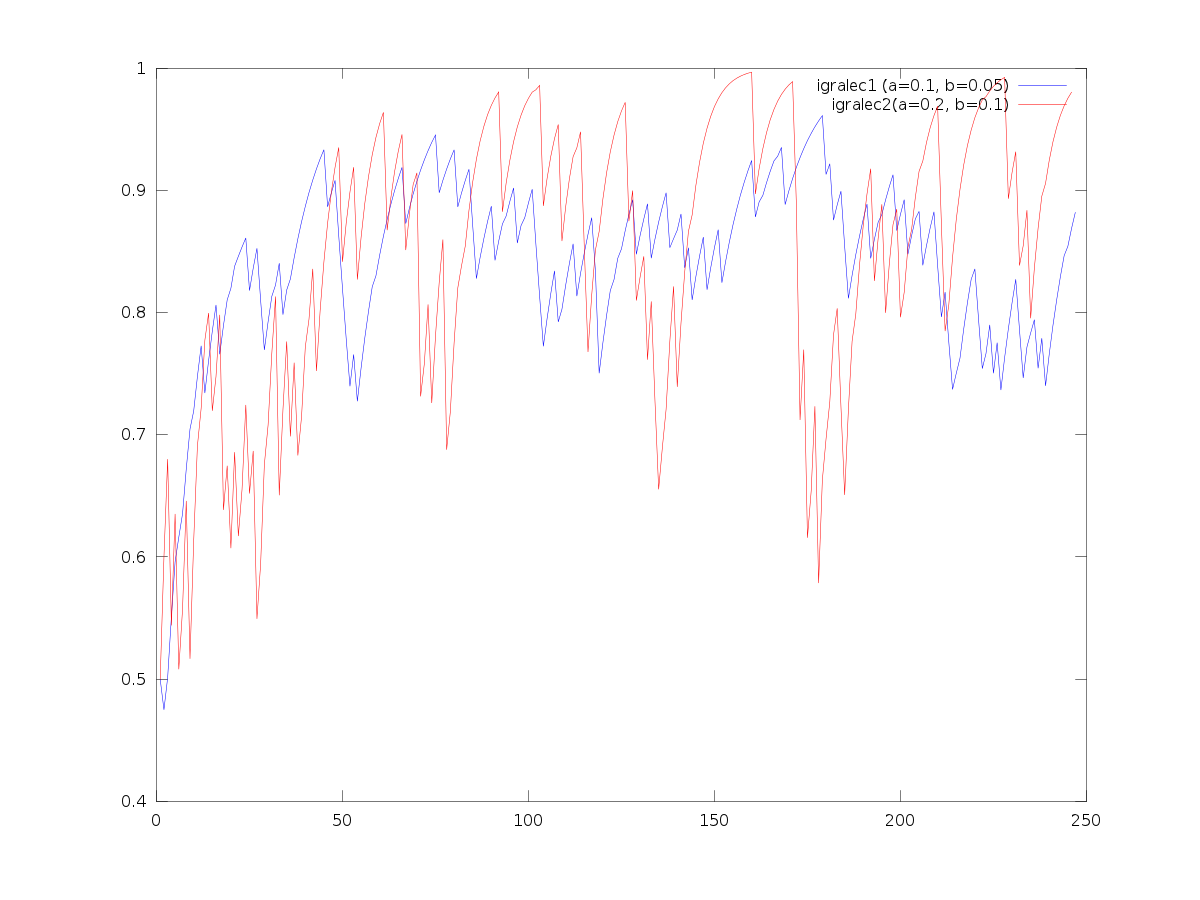
\includegraphics[scale=0.4]{fig_lrp.png} 
\end{center}
\caption{Primerjava dveh $L_{r-p}$ avtomatov z razlicnimi parametri. Graf prikazuje verjetnost izbire za avtomat ugodne akcije (za igralca 1 je to levo, za drugega desno)}
\end{figure}

\begin{figure}[h!]
\begin{center}
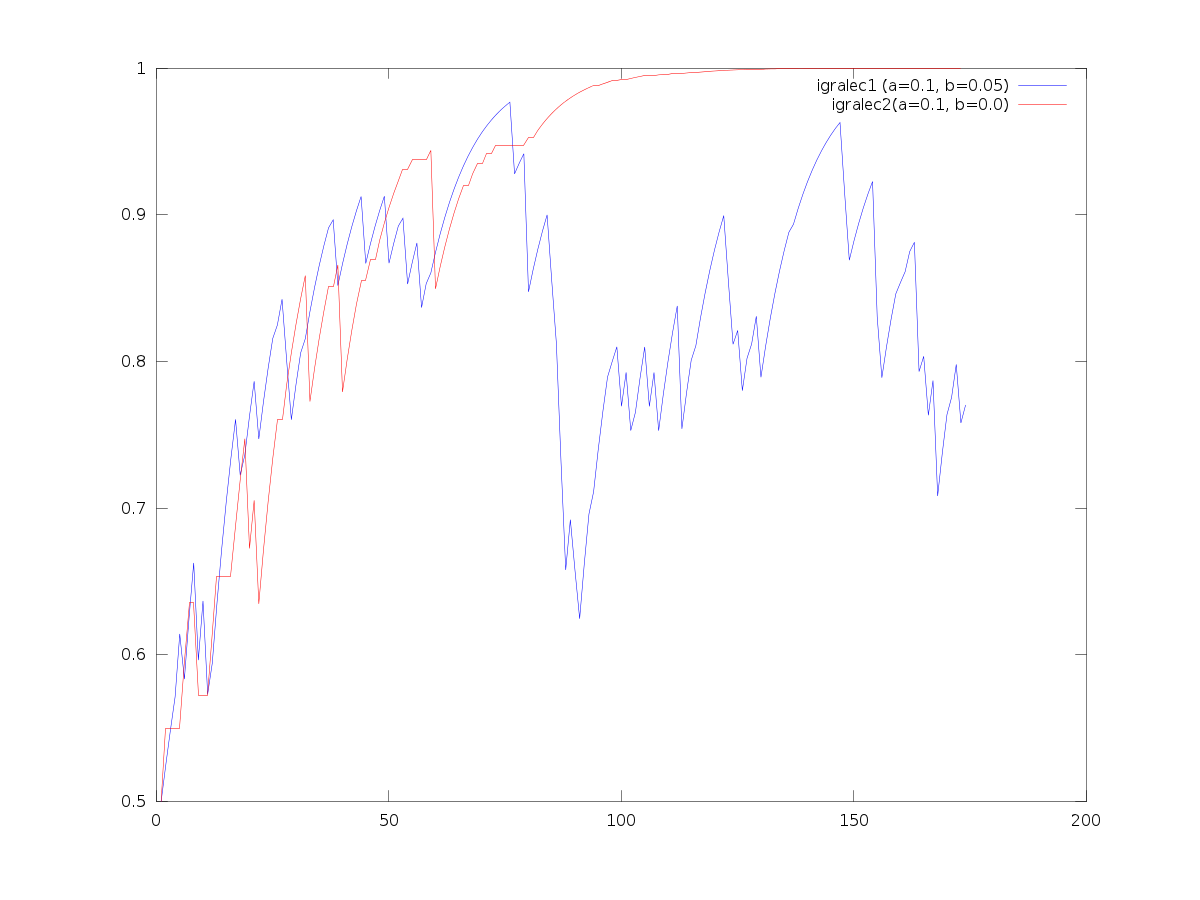
\includegraphics[scale=0.4]{fig_lrp_lri.png} 
\end{center}
\caption{Primerjava $L_{r-p}$ in $L_{r-i}$ avtomatov z enakim a. Graf prikazuje verjetnost izbire za avtomat ugodne akcije (za igralca 1 je to levo, za drugega desno)}
\end{figure}

\begin{figure}[h!]
\begin{center}
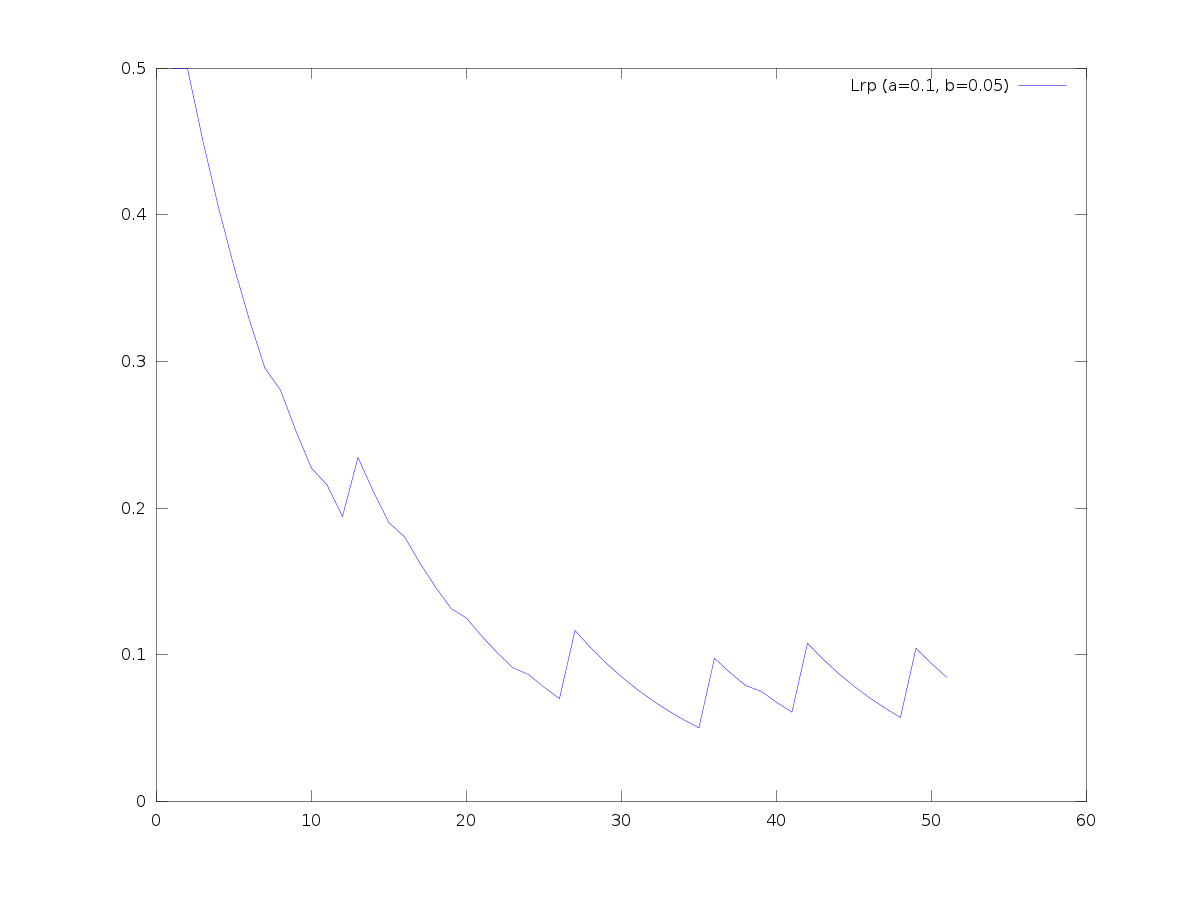
\includegraphics[scale=0.4]{lrp_pen.png} 
\end{center}
\caption{Casovna odvisnost $M(n)$ pri avtomatu $L_{r-p}$}
\end{figure}

\begin{figure}[h!]
\begin{center}
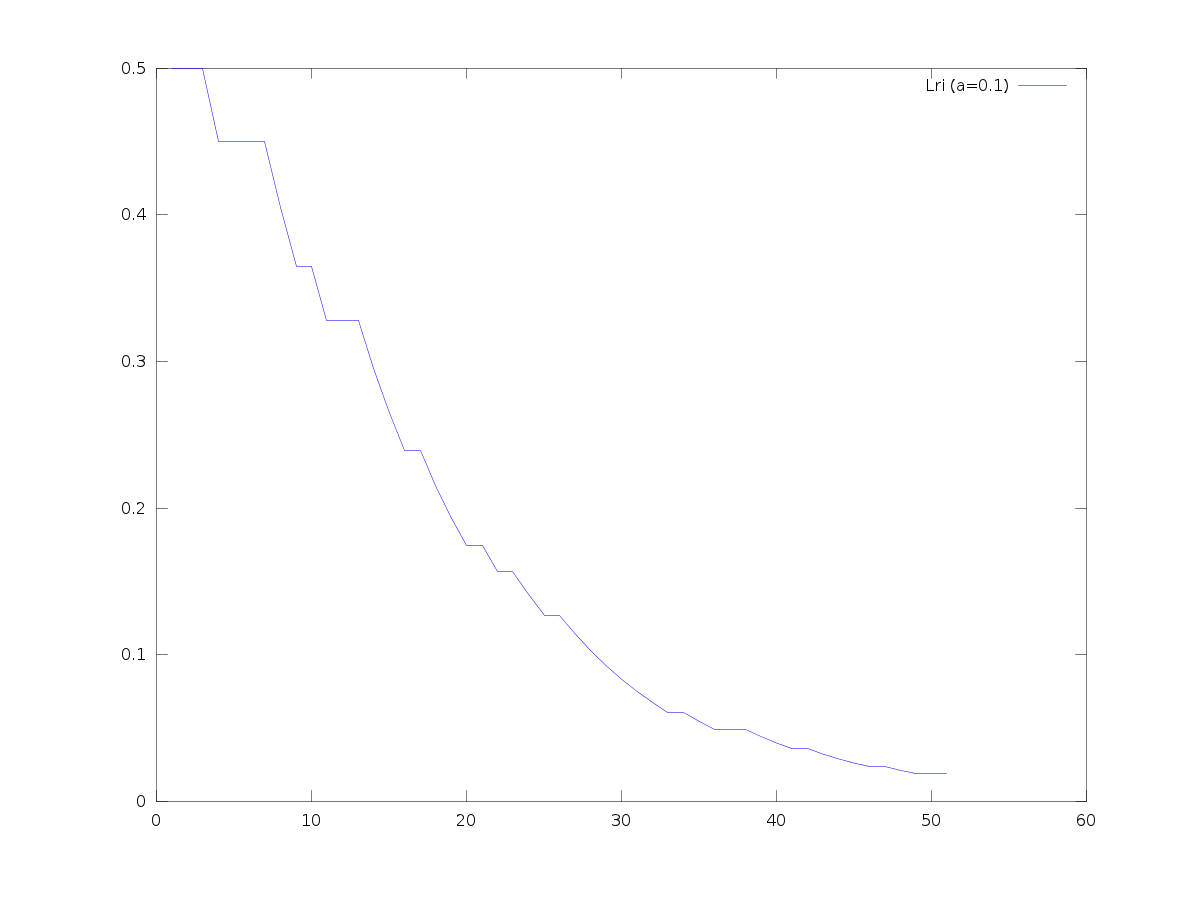
\includegraphics[scale=0.4]{lri_pen.png} 
\end{center}
\caption{Casovna odvisnost $M(n)$ pri avtomatu $L_{r-i}$}
\end{figure}

\section{Igra avtomata z clovekom}

Preizkusil sem se v igri z $L_{2n,2}$ in $L_{r-i}$ pri N=7. Za manjse N je igra za cloveka se obvladljiva in je mozno premagati avtomat v vsaj polovici primerov. Ko pa N narasca pa kolicina podatkov za cloveka postane neobvladljiva in se avtomati izkazejo dosti bolje.

\section{Zakljucek}

Predvsem se bil presenecen nad uspesnostjo avtomata $L_{2n,2}$, ki kljub svoji preprostosti kaze veliko zmoznost ucenja v tem primeru in premaguje druge, po zasnovi naprednejse avtomate. Kot drugi najboljsi se izkaze $L_{r-i}$

\end{document}